\begin{section}{Problema 3}

	\textit{Bernardo se encuentra en una prisión que consta de $n$ habitaciones conectadas por $m$ pasillos. Cada pasillo conecta exactamente $dos$ habitaciones y puede ser transitado en ambas direciones. En toda la prisión hay $p$ puertas, cada una puede abrirse con una única llave. Tanto las puertas como las llaves están repartidas en las habitaciones, de tal forma que cada habitación puede tener una única puerta o almacenar una única llave, pero no ambas cosas. Si una habitación tiene puerta, la llave correspondiente es necesaria para entrar a la habitación, independientemente del pasillo que se use para llegar a la misma. Bernardo se encuentra en la habitación $uno$, mientras que desde la habitación $n$ es posible salir de la prisión. Decidir si Bernardo puede recorrer las habitaciones recolectando llaves y abriendo puertas de manera tal de llegar a la habitación $n$ y asi escapar.}
		
	\begin{subsection}{Explicación}
		Bernardo recorre las habitaciones que tengan conexión con la habitación donde se encuentra, siempre y cuando pueda entrar, ya sea porque tiene la llave o porque la habitación no tiene puerta. Su procedimiento continúa hasta que:
		\begin{itemize}
			\item Llega a la habitación $n$, por lo tanto encontró la salida.
			\item Se le terminan los accesos a las habitaciones vecinas, es decir no puede acceder a ninguna habitación todavía no visitada y por lo tanto no puede escapar.
		\end{itemize}

	\end{subsection}

	\begin{subsection}{Detalles de la implementación}
		Modelamos este problema con un grafo donde los vértices corresponden a las habitaciones (puede ser una habitación con una llave dentro, con una puerta o sin puerta ni llave) y las aristas a los pasillos.	

		Generamos la matriz de adyacencia del grafo (de $n\times n$ donde $n$ es la cantidad de habitaciones donde cada posición $(i,j)$ de la matriz contiene un $uno$ si la habitación $i$ está conectada con la habitación $j$ y $cero$ en caso contrario). Nos referiremos a la matriz como $conexiones$.

		Para toda habitación que tenga puerta existe una llave. Poseer esta llave implica tener la posibilidad de acceder a la habitación. Podemos abstraernos del problema de Bernardo y considerar a las llaves como valores booleanos en un arreglo que nos dice para cada vértice, si este es accesible o no. Tenemos entonces, un arreglo de tipo bool ($tengo\_llave$) de tamaño $n$ donde cada vértice, representado por el índice de dicho arreglo, esta seteado en $verdadero$ si es accesible y en $falso$ sino.

		Por otro lado, tenemos un arreglo $puertas$ de tamaño $n$ (siendo $n$ es la cantidad de vértices del grafo), donde cada posición, si corresponde a una habitación con llave, tiene el vértice al cual habilita el acceso. En caso contrario, el arreglo contiene el valor $cero$. El valor es $cero$, porque como se verá más adelante en el pseudocódigo, modificará información del primer vértice, que a los fines prácticos, no modifica el resultado final del algoritmo.
		
		También tenemos un arreglo de bools llamado $enEspera$ el cual esta inicializado en falso si el vértice $i$ no puede ser accedido (tiene puerta), y en verdadero en caso contrario. Entonces, para cada vértice, de existir una posible restricción de acceso, su posición permanece en falso.

		Para la resolución del problema recorrimos el grafo de forma ordenada por niveles. Para esto hicimos una modificación al algoritmo $Breadth\; First\; Search$. La modificación consiste en visitar los vértices adyacentes al 'actual' tales que todavía no fueron visitados y tienen acceso permitido, cuando esto último no ocurre se pone el vértice en 'espera' hasta que por otro camino se encuentre al vértice que habilite el acceso al mismo. Al momento de conseguir el acceso a un vértice que se encuentra en 'espera' se lo accede directamente (sin volver a pasar por los vértices que llevan a él) considerando posible ese camino hacia el vértice $n$. Cabe destacar que este algoritmo puede acceder a cada vértice sólo una vez.

		El objetivo del $bfs$ es llegar desde el primer vértice al último.
		
		\newpage

		El siguiente pseudocódigo refleja el comportamiento previamente descripto:\VSP

		\begin{pseudo}
		\func {prision}{$conexiones, tengo\_llave, puertas, n$}
		\tab $llegue \leftarrow false$\\
		\tab $cola\; q$\\
		\tab $visitados[0..n] \leftarrow false$\\ 
		\tab $enEspera[0..n] \leftarrow false$\\ 
		\tab $encolar(q,0)$\\
		\tab $visitados[0] \leftarrow true$\\
		\tab \WHILE $!esVacia(q) \AND !llegue$\\
		\tab \tab $actual \leftarrow primero(q)$\\
		\tab \tab $desencolar(q)$\\
		\tab \tab \FOR $ i\leftarrow0 \TO n \AND !llegue$\\
		\tab \tab \tab \IF	$conexiones[actual][i] \AND tengo\_llave[i] \AND !visitados[i]$\\
		\tab \tab \tab \tab	$tengo_llave[puertas[i]] \leftarrow true$\\
		\tab \tab \tab \tab	$encolar(q,i)$\\
		\tab \tab \tab \tab	$visitados[i] \leftarrow true$\\
		\tab \tab \tab \tab	$llegue \leftarrow (i == n-1)$\\
		\tab \tab \tab \tab \IF	$enEspera[puertas[i]]$\\
		\tab \tab \tab \tab \tab $encolar(q,puertas[i])$\\
		\tab \tab \tab \tab \tab $visitados[puertas[i]] \leftarrow true$\\
		\tab \tab \tab \tab \tab $llegue \leftarrow (n-1==puertas[i])$\\
		\tab \tab \tab \ELSE \\
		\tab \tab \tab \tab \IF $conexiones[actual][i] \AND !visitados[i]$\\
		\tab \tab \tab \tab \tab $enEspera[i] \leftarrow true$\\
		\tab \RET $llegue$\\
		\end{pseudo}

		En pocas palabras, la idea del algoritmo es explorar el grafo con $bfs$ en busca de un camino que inicie en el vértice $cero$ y llegue al vértice $n$, si se encuentra con un vértice que no es accesible, espera hasta que desde otro camino se habilite la entrada a ese vértice, una vez habilitada continua por ese camino, mientras sigue recorriendo todo camino que se encuentre habilitado hasta el momento.

		El resultado final viene dado por la variable $llegue$. Es inicializada en $falso$ y se setea en $verdadero$ si sólo si en algún momento el vértice a encolar es el $n$ ($i == n-1$), es decir, el vértice $n$ fue alcanzado por el $bfs$. Si esto ocurre, podemos concluir que pudimos llegar al vértice objetivo. Si pasa por todos los vértices habilitados y los que pudo habilitar y no puede llegar al vértice $n$, sale del ciclo (\textbf{while}) sin cambiar el valor de $llegue$ y devuelve $falso$.
		
	\end{subsection}


	\begin{subsection}{Análisis de complejidad}
		Como mencionamos previamente, el algoritmo \textbf{no} podrá pasar más de una vez por cada vértice. Mientras quede algun vértice por ver y pueda accederse, seguirá intentando llegar al nodo $n$. Analizando la complejidad, vemos que si el $bfs$ pudiera acceder indistintamente a todos los vértices del grafo, el ciclo $while$ tendría un costo de $n$ iteraciones.
		
		Dentro del ciclo principal tenemos las primeras dos operaciones con costo constante (una asignación y quitar de la pila el primer elemento), y un ciclo anidado ($for$).
		
		Por lo tanto tenemos hasta el momento $n$ interaciones del ciclo $while$ donde dentro de él tenemos un ciclo $for$. Una primer aproximación a la complejidad final sería pensar que para cada una de las $n$ iteraciones tendremos un costo $h$ todavía no conocido por el ciclo $for$, descartando para complejidad el costo constante de la asignación y quitar el primer elemento de una pila. Tenemos hasta ahora, \Ode{n*h}.
		
		Analizemos ahora la cantidad de operaciones a la que equivale $h$ en el peor caso.
		
		El ciclo $for$ itera en el peor caso desde $0$ hasta $n$ (puede salir antes si el valor de la variable bool $llegue$ se setea en verdadero). Por lo tanto tenemos que $h$ será a lo sumo $n*c$ porque dentro de este ciclo anidado, se asignan valores a arreglos, matrices, se encolan parámetros constantes a pilas, se setean valores booleanos y se chequea guardas de condicionales $if$ siendo todas estas operaciones, de costo constante. Cabe aclarar que la cantidad de veces que se realizan estas operaciones por cada iteración también es constante, por lo que se puede deducir que una iteración del ciclo $for$ tiene costo constante. Es así entonces que $h = n*c$ (con $c$ constante).
		
		Continuando con el análisis de complejidad, teníamos que el algoritmo tenia complejidad de \Ode{n*h}, siendo ahora $h=n*c$. Por lo tanto, la complejidad de este algoritmo es \Ode{n*n*c} = \Ode{n^2} $\subset$ \Ode{n^3}
	\end{subsection}


	\begin{subsection}{Pruebas y Resultados}
		Para probar correctitud contamos con un generador de instancias en las cuales Bernardo puede escapar y otras en las cuales no, que nos devuelve un archivo $test\_libre.in$ y $test\_no.in$ respectivamente. De esta forma, con una comparación de archivos (comando \texttt{make diffs} en la carpeta Ej3) podemos saber para cada instancia si el resultado obtenido por nuestro algoritmo es correcto.

		Para analizar la complejidad temporal del algoritmo (cantidad de operaciones) tenemos un generador aleatorio de 'mapas' donde para cada número de habitaciones $n$ variamos el porcentaje de pasillos con respecto al máximo (es decir, variamos la densidad del grafo). Generamos para cada $n$ desde $4$ a $100$ ($4$ por enunciado y $100$ porque nos pareció suficente para comprobar el comportamiento del algoritmo), $10$ casos con densidad $0.3$ y $0.6$ y $0.9$. También, generamos mejores casos, en donde la habitación $1$ no está conectada por ningún pasillo a otra. El algoritmo necesita por lo menos, buscar entre todos los vértices los adyacentes al primero (la habitación de la que sale Bernardo) para poder afirmar que no tiene ninguno y terminar (para toda instacia, el algoritmo necesita de la inicialización de dos arreglos, previo a entrar al ciclo $while$). Deducimos que el costo para estos casos es lineal.

		\newpage

		A continuación se muestra para cada instancia la cantidad de operaciones en función de la cantidad de habitaciones y la cantidad de pasillos (densidad del grafo). Esperamos ver que cuánto mayor es la densidad mejor es el algoritmo.
		
		\gra{prision/count_test_densidades.pdf}

		Podemos ver que se cumple lo predicho ya que para un $n$ fijo (para una cantidad de habitaciones fija), la función crece (la cantidad de operaciones aumenta) conforme disminuye la cantidad de pasillos. 
		Además, vemos que cuanto mayor es la densidad más tienden a agruparse, consideramos que esto pasa porque a que a medida que aumenta la densidad la variedad de instancias posibles disminuye, siendo alta la probabilidad de que se repitan al generarlas y siendo las distintas configuraciones del grafo muy similares con respecto al costo.\VSP

		\newpage

		Por otro lado, generamos peores casos para el algoritmo $\forall n\; (4 \leq n \leq 100)$. Para generarlos, armamos un árbol donde la raíz es la habitación  $uno$. La cantidad de llaves/puertas es exactamente $\lfloor \frac{(n-2)}{2}\rfloor$ . Si $n$ es par, en el nivel $uno$  están todas las habitaciones con puerta y otra que tiene la llave de la habitación $\frac{(n-2)}{2} + 1$ . En el nivel $dos$ están el resto de las habitaciones, es decir, las habitaciones que tienen las llaves y la última habitación. Si $n$ es impar, en el nivel $uno$  están todas las habitaciones con puerta y otra que no tiene llave ni puerta. En el nivel $dos$ están el resto de las habitaciones, es decir, las habitaciones que tienen las llaves y la última habitación. En ambos casos, la llave correspondiente a la habitación $i$, $\forall i (2 \leq i \leq \frac{(n-2)}{2})$ está en la habitación $n-i+1$. Este tipo de mapa es uno de los peores casos del algoritmo porque para determinar que puede escapar, el $bfs$ visita necesariamente todos los nodos, dejando en espera a todos los bloqueados para luego visitarlos.

		La siguiente figura muestra lo descripto anteriormente para $n$ par, siendo la habitación $2$ la que contiene la puerta uno:
	
		\begin{center}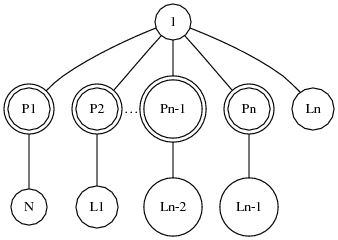
\includegraphics[width=9cm]{prision/peor_caso.png}\end{center}

		\begin{itemize}
		\item La letra 'P' se refiere a 'puerta'.
		\item La letra 'L' se refiere a 'llave'.
		\item '1' se refiere a la habitación en la que Bernardo inicia.
		\item 'N' se refiere a la habitación por la que Bernardo podría escapar de la prisión.
		\end{itemize}

		\newpage

		La siguiente figura muestra lo descripto anteriormente para $n$ impar, siendo la habitación $2$ la que contiene la puerta uno:

		\begin{center}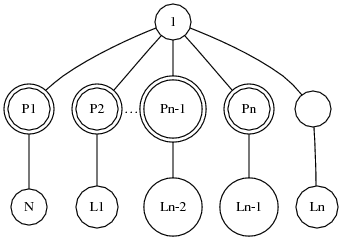
\includegraphics[width=9cm]{prision/peor_caso_impar.png}\end{center}

		\newpage

		En el siguiente gráfico se muestra la cantidad de operaciones en función de la cantidad de habitaciones y la cantidad de pasillos (densidad del grafo). Ademas, graficamos la función $19*n^2$ ya que es la cota superior previamente calculada con una constante aproximada calculada empíricamente. El objetivo de esta prueba es poder constrastar los casos del gráfico anterior con los peores casos y mejores caso para el algoritmo, para corroborar que las cotas son correctas. 
		
		\gra{prision/count_test_peor_caso.pdf}

		Se puede ver que $19*n^2$ es la cota superior exacta para el algoritmo. Además, podemos afirmar que las instancias elegidas como peores casos se comportan como tal. En general, vemos que el algoritmo se comporta mucho mejor que la cota. Hicimos $1000$ test aleatorios por cada densidad y la cantidad de operaciones no superó las $40000$ en ninguno de ellos. En cambio los peores casos superan esta cantidad de operaciones con $n$ a partir de $45$ aproximadamente. Podemos concluir que cuanto mayor sea $n$, mayor será la diferencia de $performance$ entre el peor caso y los elegidos aleatoriamente (con la salvedad de que no se elija un peor caso).

		Vemos que la cantidad de operaciones para los mejores casos crece linealmente como habíamos supuesto. Creemos entonces que la cota inferior para el algoritmo fue bien elegida.

		Vale observar que no tomamos en cuenta el costo de la inicialización de la matriz de adyacencia (su costo es $n^2$), de esta forma podemos afirmar que nuestro mejor caso para la función ciudad es lineal (la complejidad se analizó sólo sobre la función principal -ciudad-).

		
	\end{subsection}

	\begin{subsection}{Conclusiones}
		Modelar el problema con un grafo, permitió abstraernos de Bernado y la prisión, pudiendo pensar en técnicas para recorrerlos de forma eficiente. Así, realizar un $bfs$ sobre nodos (un algoritmo conocido) con cambios mínimos, satisfizo los requerimientos del problema.

		Habiéndolo modelado con grafos y recorrido de forma ordenada, pudimos implementar un algoritmo polinomial de complejidad $n^2$. Podemos concluir que el problema está computacionalmente 'bien' resuelto.

		Al tener muchas variables en el problema, como la cantidad de habitaciones, pasillos, llaves y el lugar donde estas estaban, complejizaron la realización de los gráficos. Terminamos realizando test con cantidad de habitaciones fijas, cantidad de pasillos fijos (la máxima cantidad de pasillos posibles para esa cantidad de habitaciones multiplicaba por una densidad entre 0 y 1) siendo aleatorios los extremos (las habitaciones que conectan), y llaves distribuídas de forma también aleatoria. Creemos que de esta forma, al realizar una cantidad significativa de tests, cubrimos una cantidad suficiente de casos.

	\end{subsection}
\end{section}

